\subsection{Particle Gibbs}
Here, we follow the Particle Gibbs algorithm described in Algorithm~\ref{alg:sampling/pmcmc-pg-pg/pg}. The illustrations are below in Figure~\ref{fig:pprog/how/figures/pgibbs1}, and Figure~\ref{fig:pprog/how/figures/pgibbs2}. Whenever a \verb!predict! is needed, a sample of the posterior of the execution trace can be obtained by sampling from
\begin{equation*}
	\hat p(\mathrm d \vec x_n \mid y_{1:n}, \vec \theta) = \sum_\ell \hat w_n^{(\ell)} \delta_{\vec x_n^{(\ell)}}(\mathrm d \vec x_{n})
\end{equation*}
(This is \emph{with} the retained particle).

\begin{figure}[!htb]
\centering
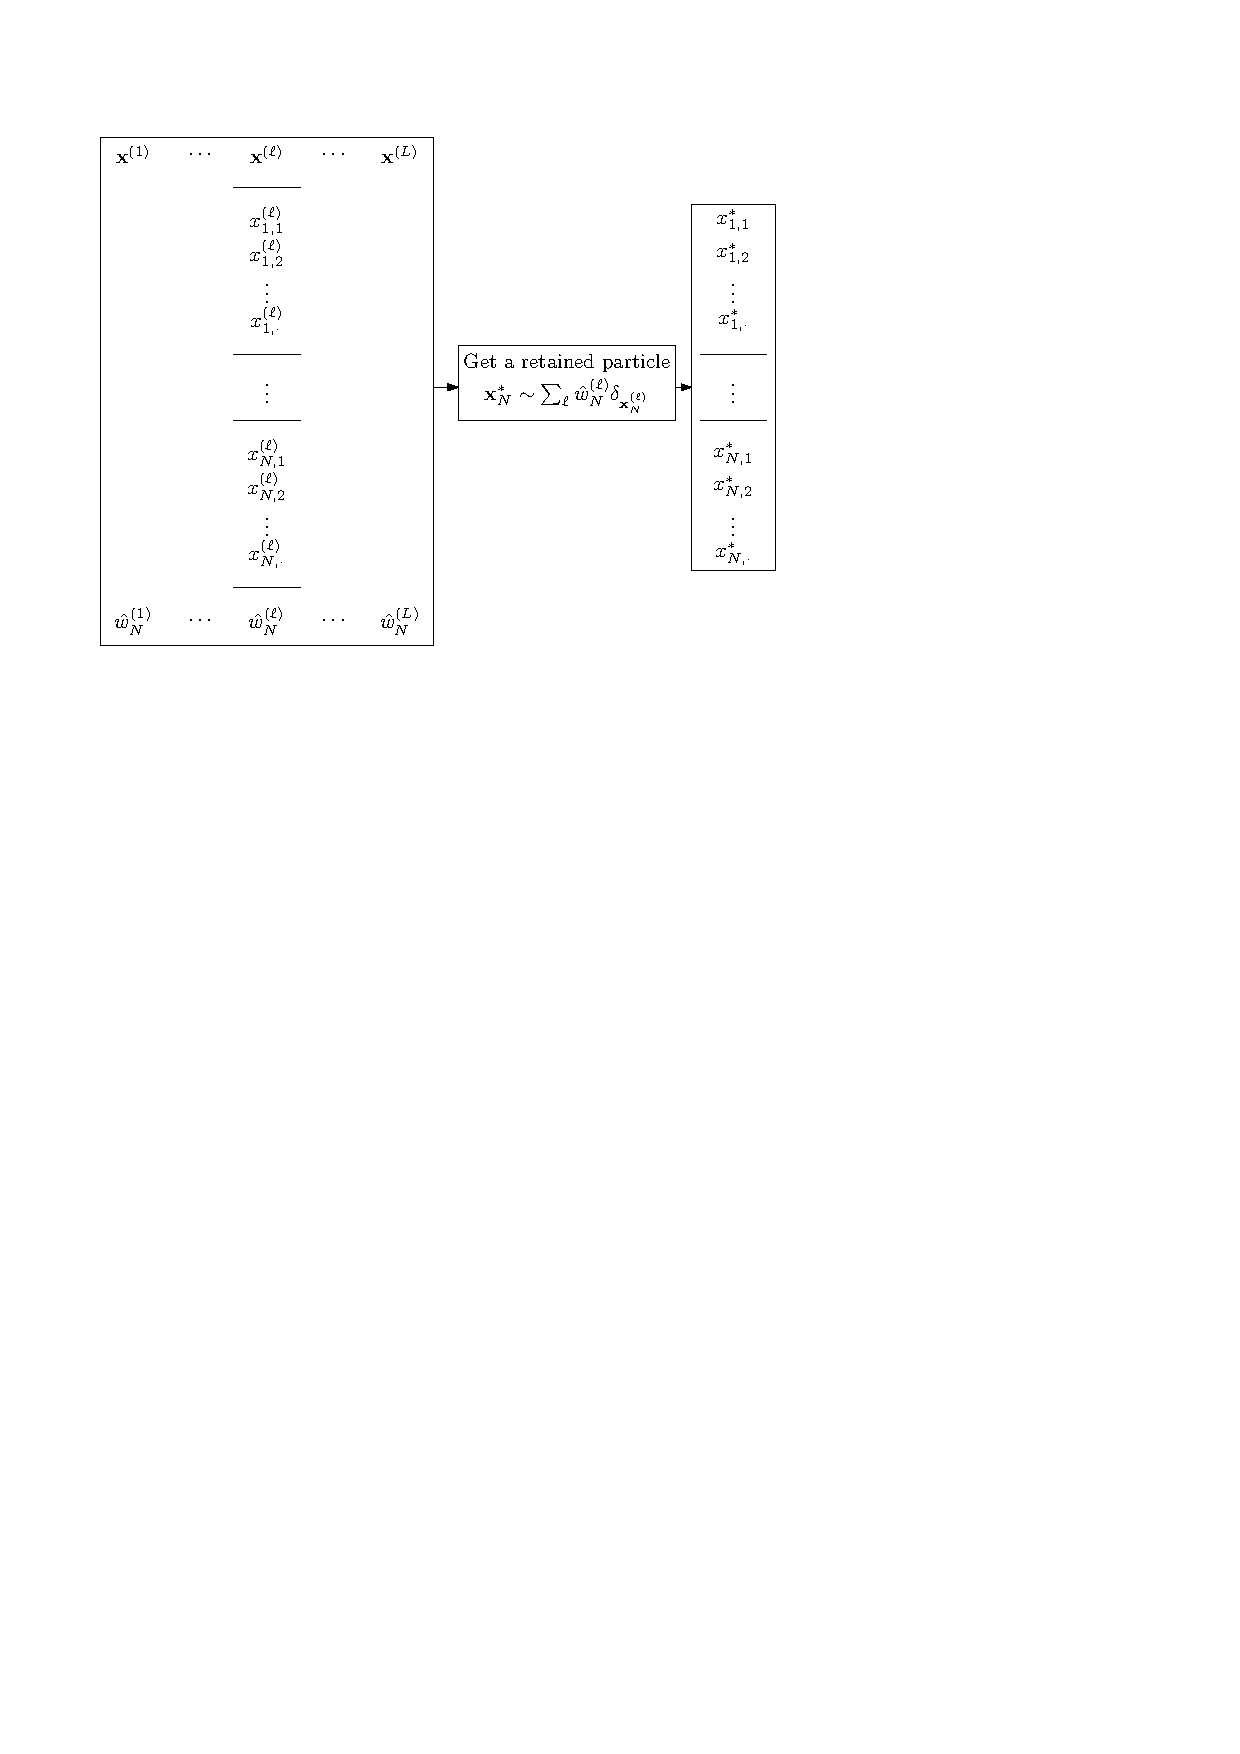
\includegraphics[scale=0.75]{pprog/how/figures/pgibbs/pgibbs1}
\caption{Initialisation of the Particle Gibbs sampler.}
\label{fig:pprog/how/figures/pgibbs1}
\end{figure}

\begin{figure}[!htb]
\centering
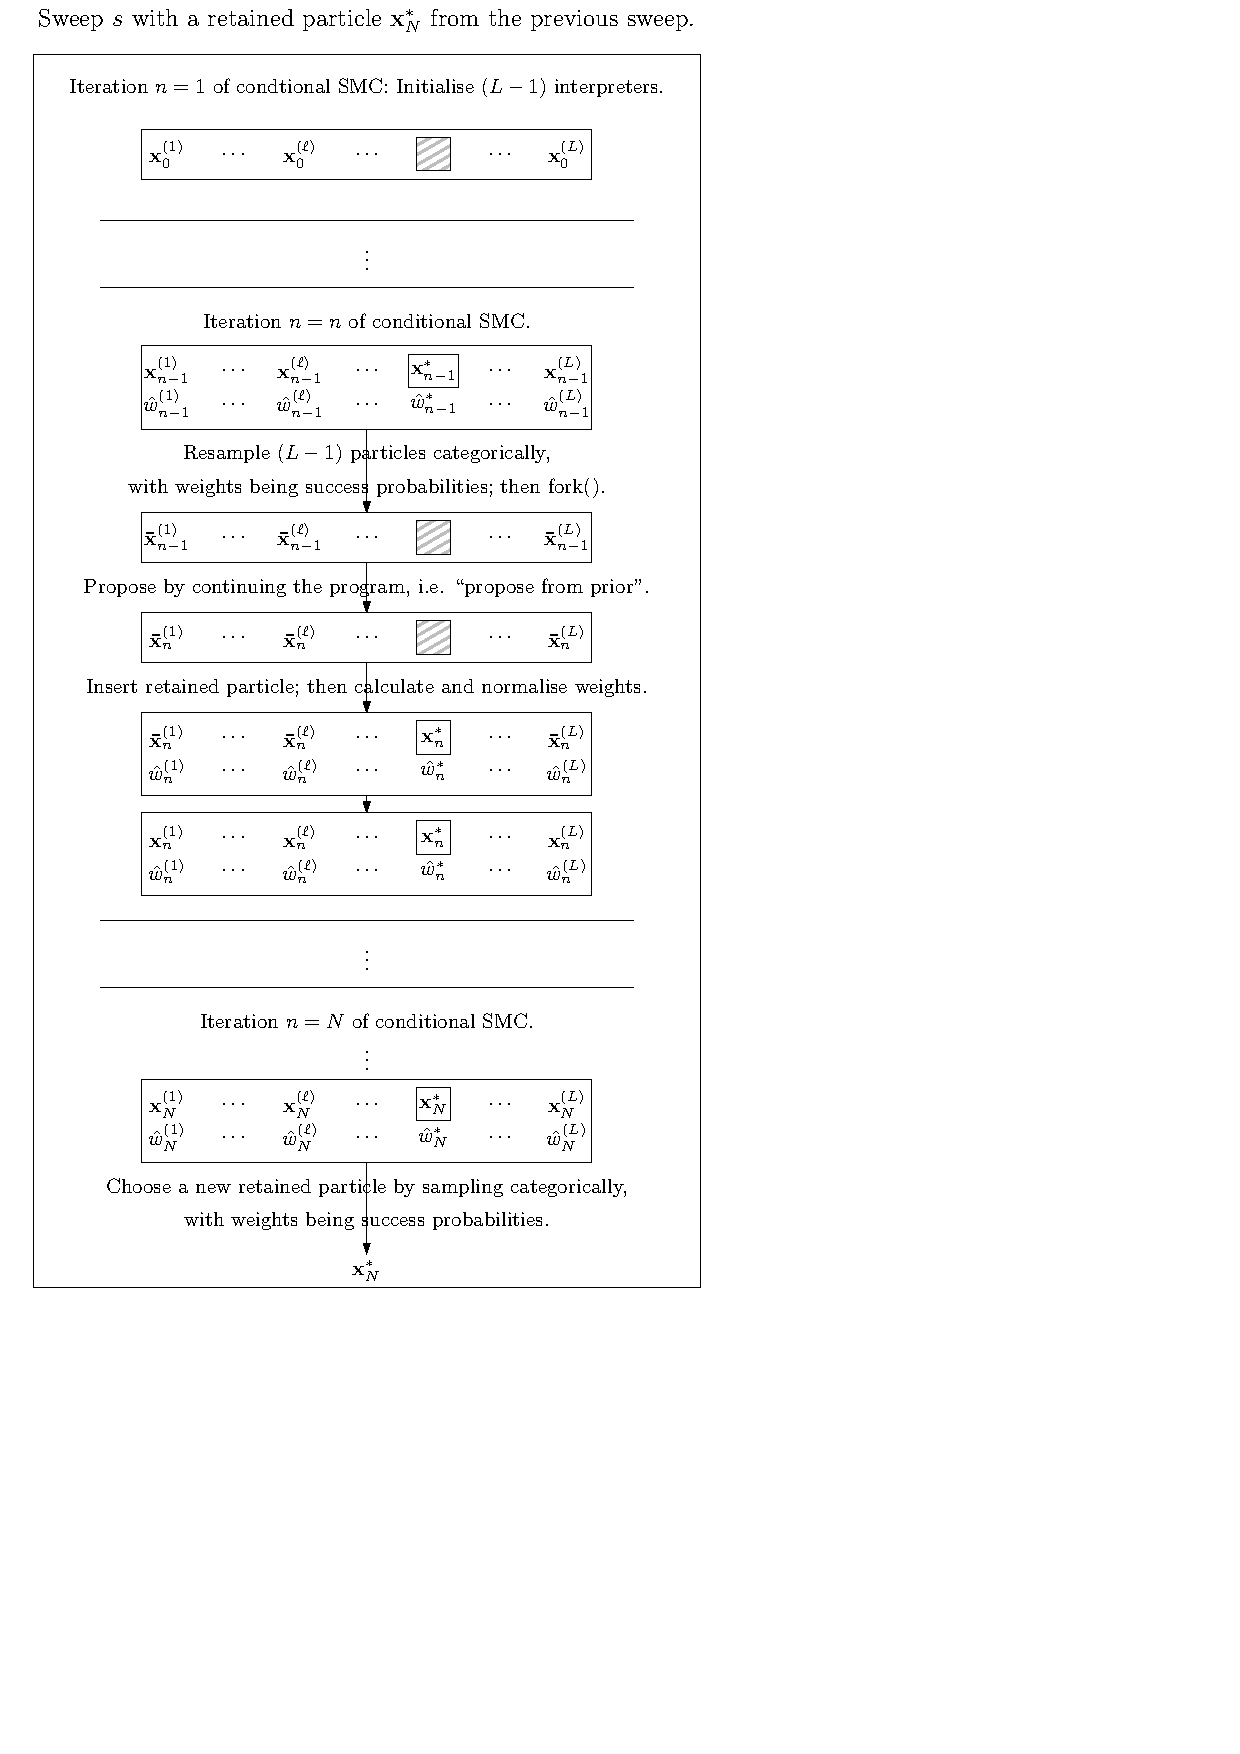
\includegraphics[scale=0.8]{pprog/how/figures/pgibbs/pgibbs2}
\caption{Sweep $s$ of the Particle Gibbs sampler.}
\label{fig:pprog/how/figures/pgibbs2}
\end{figure}